% SASYR 2025 - Template based on:
% The samplepaper.tex, a sample chapter demonstrating the
% LLNCS macro package for Springer Computer Science proceedings;
% Version 2.20 of 2017/10/04

\documentclass[runningheads]{llncs}

% Graphics and related packages
\usepackage{graphicx}
\usepackage{lipsum}
\usepackage{url}
% Uncomment the line below if using the hyperref package for URL formatting
% \renewcommand\UrlFont{\color{blue}\rmfamily}

% Math and symbols packages
\usepackage{amssymb}
\usepackage{amsmath}

% Captioning packages for figures
\usepackage{caption}
\usepackage{subcaption}

% Additional symbols package
\usepackage{gensymb}

% URL font definition
\def\UrlFont{\rmfamily}

\begin{document}
%
\title{Development of a 2-DoF Antenna Radiation Measurement System}

%
\titlerunning{Development of a 2-DoF Antenna Radiation Measurement System}  
%
\author{Mauro da Silva Leme\inst{1}\orcidID{0009-0001-4945-8907} \and J. A. B. Coelho\inst{2}\orcidID{0009-0004-8278-7579} \and João Paulo Coelho\inst{1,2}\orcidID{0000-0002-7616-1383}}

%
\authorrunning{M. Leme et al.} 
\tocauthor{Mauro da Silva Leme, J. A. B. Coelho, João Paulo Coelho}
%
\institute{Instituto Politécnico de Bragança, Campus de Santa Apolónia, 5300-253 Bragança, Portugal;\\
\and
CeDRI, SusTEC, Instituto Politécnico de Bragança, 5300-253 Bragança, Portugal
\\
\email{a52965@alunos.ipb.pt,\{joaocoelho,jpcoelho\}@ipb.pt}
}
%
\maketitle             
%
\begin{abstract}
Understanding antenna radiation patterns is crucial for optimizing wireless communication systems. Although simulation tools predict radiation patterns during development, environmental conditions in real-world settings substantially influence outcomes. Commercial measurement systems, though precise, are often prohibitively expensive for education. This work presents a low-cost, two-axis computerised system for measuring antenna radiation patterns at 868 MHz, integrating Arduino-based control, stepper motors, and power sensors. Tested with a Yagi-Uda antenna, it yields results consistent with simulations, serving as a practical tool for telecommunications classes. By enabling real-time visualization, this mechatronic platform enhances student understanding of antenna behaviour. Designs will be shared openly to support replication.
\keywords{Antenna Pattern Analysis, Wireless Systems, Mechatronic Education, Telecommunications Training}
\end{abstract}
%

\section{Introduction and System Overview}
Antenna radiation patterns are essential in wireless communication engineering, defining signal coverage, interference, and system performance\cite{balanis2016antenna}. Simulation software predicts these patterns, yet real-world conditions, such as environmental interference and manufacturing variations, often yield different results\cite{6157745}. Accurate measurements are thus critical for validating designs. Commercial measurement systems, while precise, are prohibitively expensive and complex for educational settings, limiting students to theoretical studies and simulations~\cite{Simanjuntak2019}. This restricts hands-on learning, making electromagnetic concepts harder to grasp and reducing practical problem-solving opportunities.

To address this challenge, as shown in Figure \ref{fig:sys}, this work introduces a cost-effective, automated system for measuring antenna radiation patterns. The mechatronic platform uses Arduino-driven NEMA 17 stepper motors(1.8$^{\circ}$ resolution) and an RF power detector(based on the AD8313 integrated circuit) for dual-axis antenna rotation, with MATLAB\footnote{A campus version of this software is licensed to the Polytechnic Institute of Bragança.} visualisation. Designed in SolidWorks\footnote{Educational version licensed to the Polytechnic Institute of Bragança.}, for telecommunications education, it enables students to analyse real-world patterns, fostering practical skills. This approach bridges theoretical knowledge with experimental practice, enhancing classroom learning.
\begin{figure}
    \centering
    \begin{subfigure}{0.249\textwidth}
        \centering
        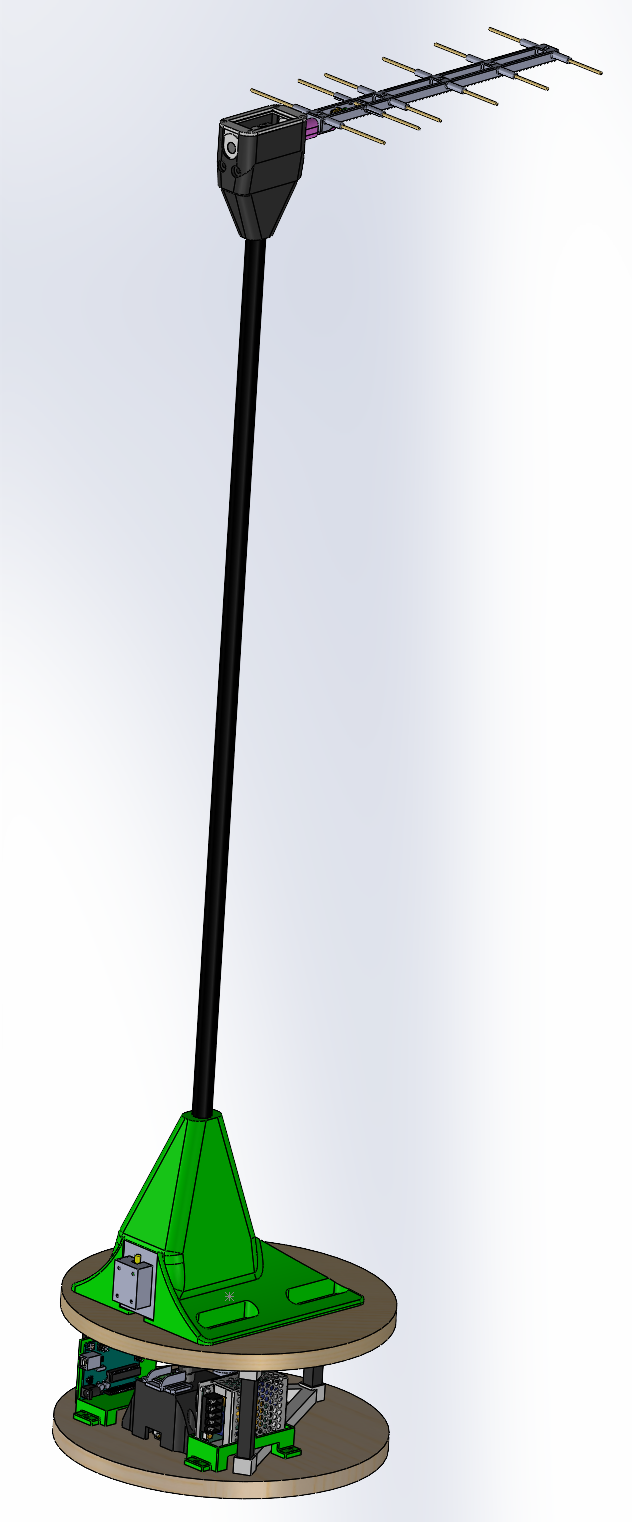
\includegraphics[width=\textwidth]{Figures/full_system.png}
        \caption{CAD rendering}
    \end{subfigure}
    \hspace{3mm}
    \begin{subfigure}{0.275\textwidth}
        \centering
        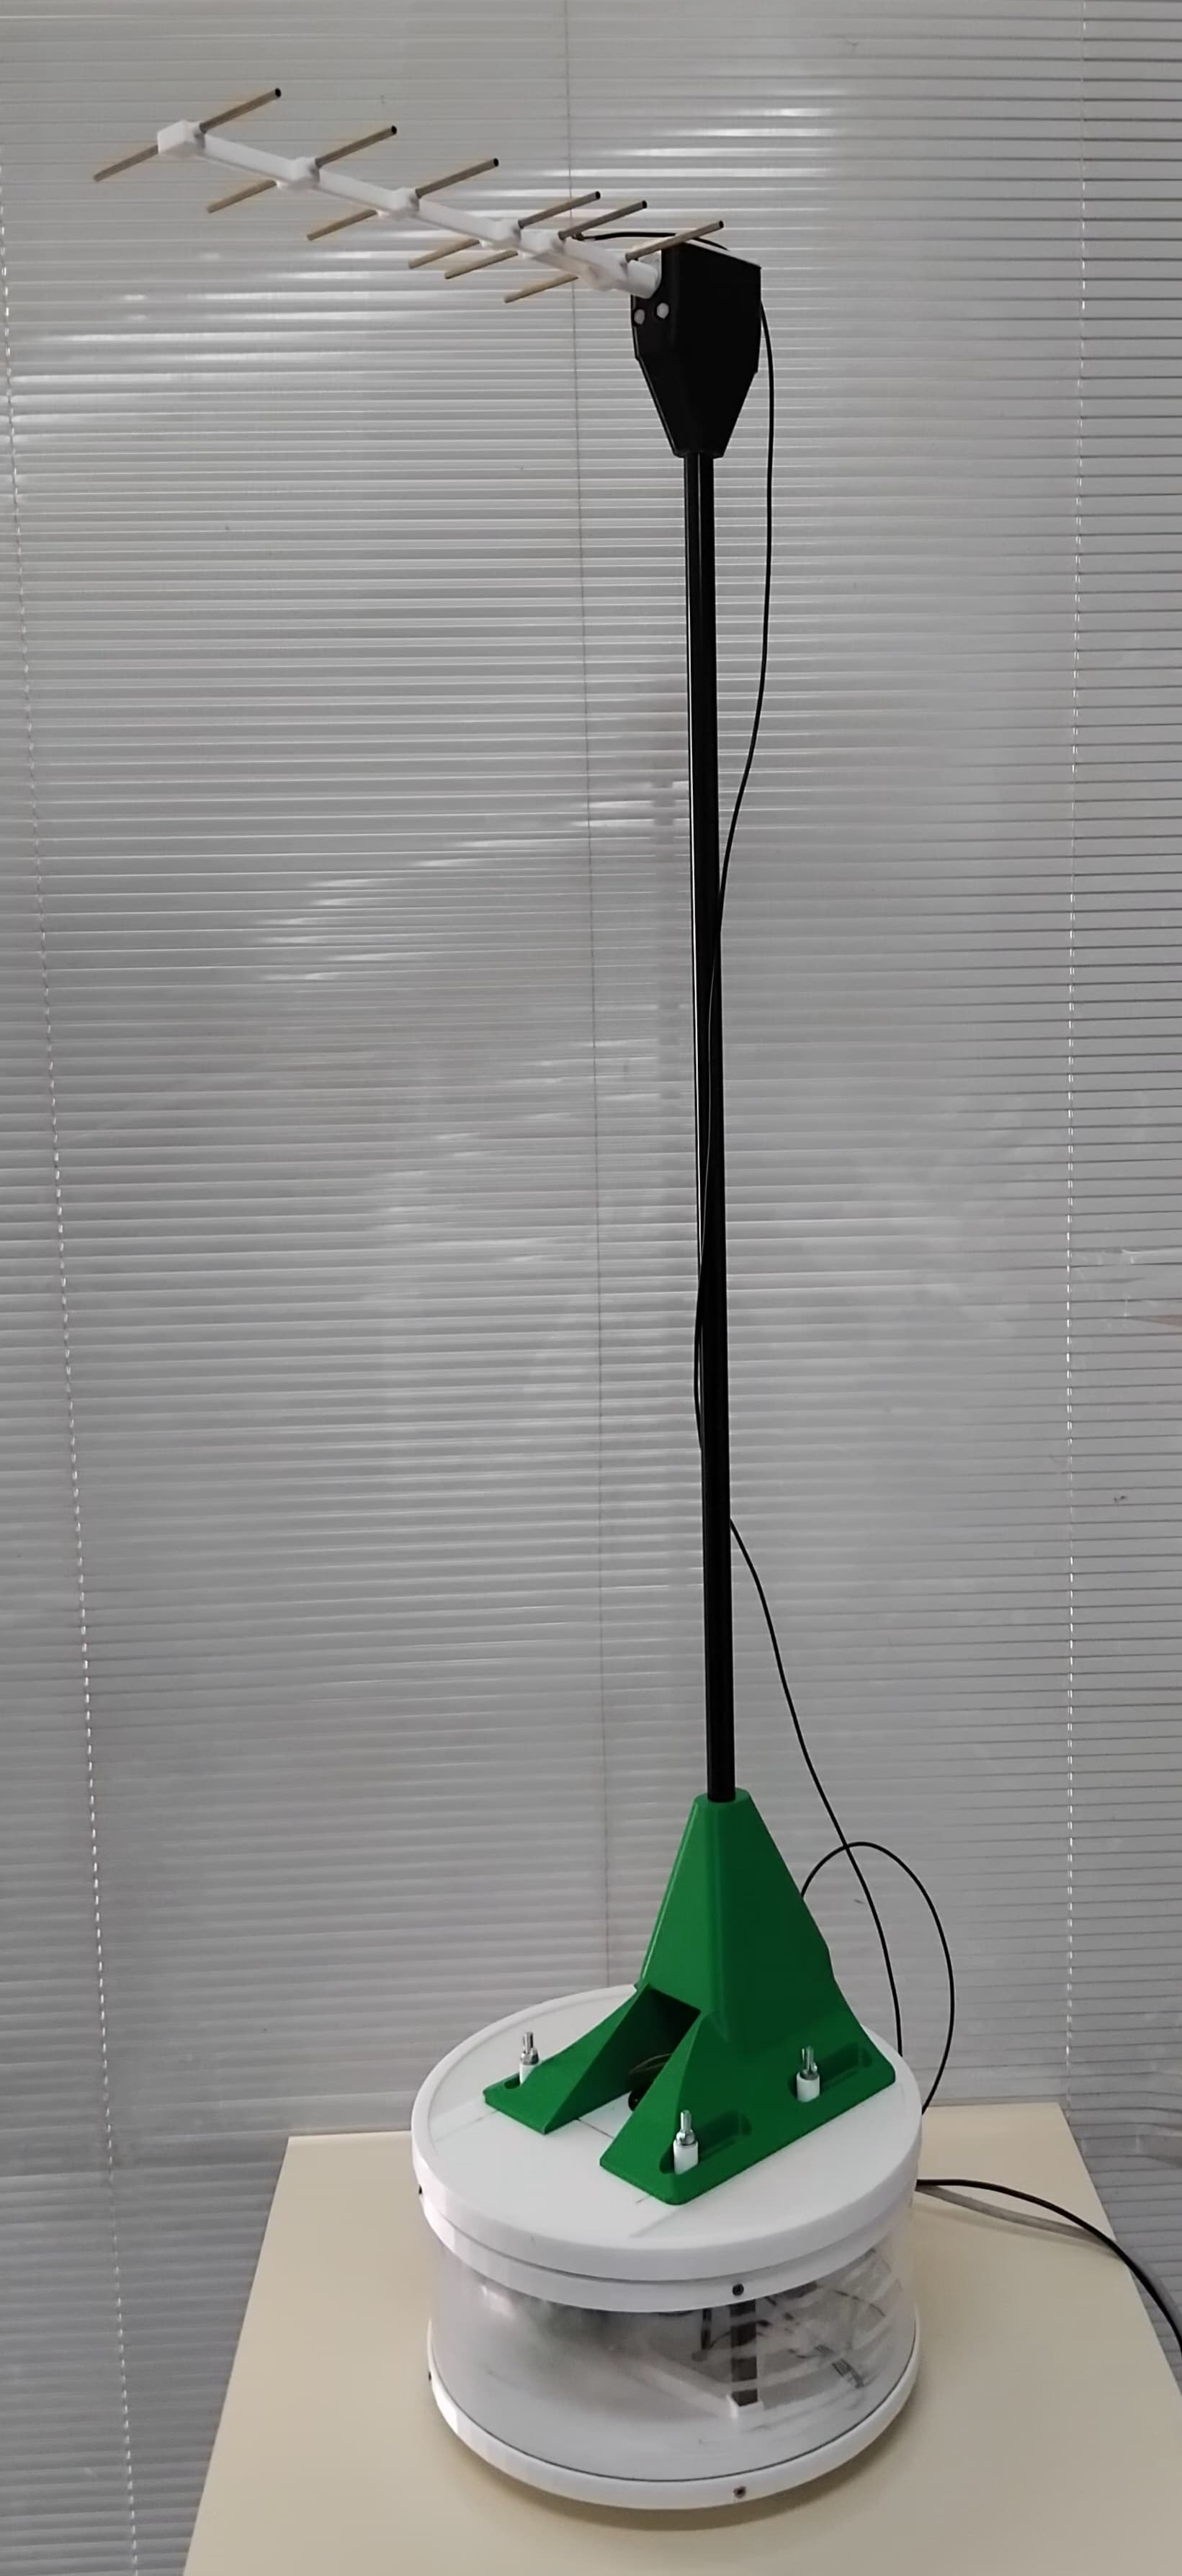
\includegraphics[width=\textwidth]{Figures/front_view_antenna.jpg}
        \caption{Physical prototype}
    \end{subfigure}
    \caption{System for antenna pattern measurement: SolidWorks (left) and assembled (right).}
    \label{fig:sys}
\end{figure}


\section{Results and Conclusion}
The system was evaluated using a Yagi-Uda antenna at 868 MHz, with its measurements compared to CST Studio Suite\footnote{The free educational version of this software was used in the simulations.} simulations. Figure \ref{sec4:fig1} illustrates the system’s ability to capture radiation patterns, closely aligning with simulated outcomes. The primary lobe was detected at 90°, with a 3 dB beamwidth of 49.08°, near the simulated 53.5°, and front-to-back ratio reduced by 17.01 dB, compared to 16.3 dB theoretically. The noise limits of the RF detector were considered.

\begin{figure}[htb!]
     \centering
     \begin{subfigure}{0.32\textwidth}
         \centering
         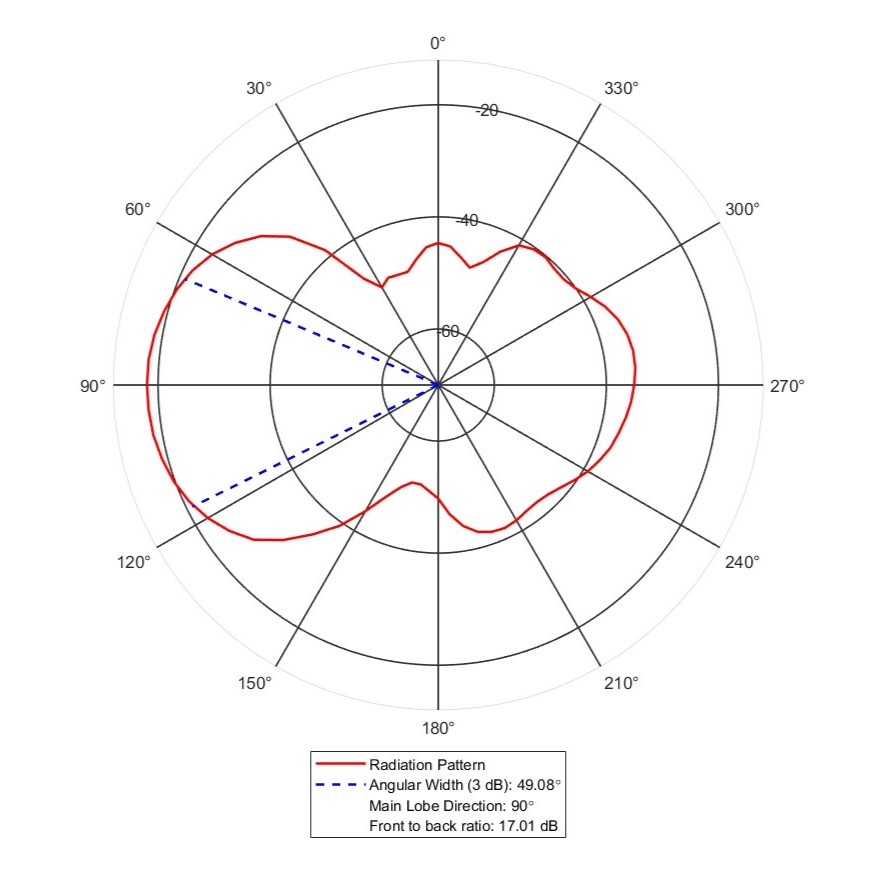
\includegraphics[width=\textwidth]{Figures/Real_data_acquired.jpg}
         \caption{Measured data}
         \label{sec4:fig1:a}
     \end{subfigure}
     \hspace{1mm}
     \begin{subfigure}{0.38\textwidth}
         \centering
         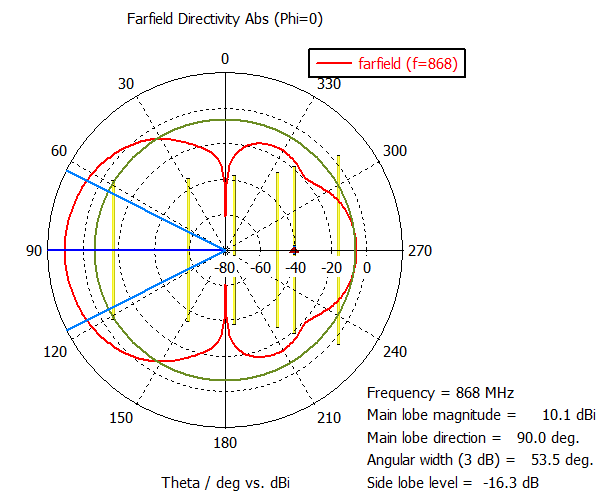
\includegraphics[width=\textwidth]{Figures/radiation_pattern_simulation.png}
         \caption{Simulated outcome}
         \label{sec4:fig1:b}
     \end{subfigure}
        \caption{Measured and simulated radiation patterns.}
        \label{sec4:fig1}
\end{figure}

Small variations, due to real-world conditions like reflections and stray signals, appeared between measured and simulated patterns, underscoring difficulties in non-ideal test settings. Though external noise impacted precision, the system consistently captured radiation patterns, proving its value for classroom learning,  even with its limitation. This reliability supports its role as an effective tool for teaching antenna concepts in educational environments.

Planned enhancements include filters to block unwanted signals, a balun to stabilize transmission, and optimized impedance alignment. Digital tutorials will be created to spark student interest in antenna principles through interactive visualizations. Sharing system designs openly will encourage collaborative improvements, strengthening its utility as an affordable platform for hands-on telecommunications education and fostering innovation.

\section*{Acknowledgment}
This work was supported by national funds: UID/05757 - Research Centre in Digitalization and Intelligent Robotics (CeDRI); and SusTEC, LA/P/0007/2020 (DOI: 10.54499/LA/P/0007/2020).


\bibliographystyle{unsrt}
\bibliography{lib/refs}
%
\end{document}
